\subsection{MetaPath}
\subsubsection{Run pathway analysis}

After opening the MetaPath page, as shown in Figure \ref{fig:MetaPathmainpage}, there are 3 main steps to implement MetaPath. We generally suggest users not to change any parameter setting in ``Advanced"  and ``Advanced Options" unless users know the underlying methodology well. 

\begin{figure}[H]
\begin{center}
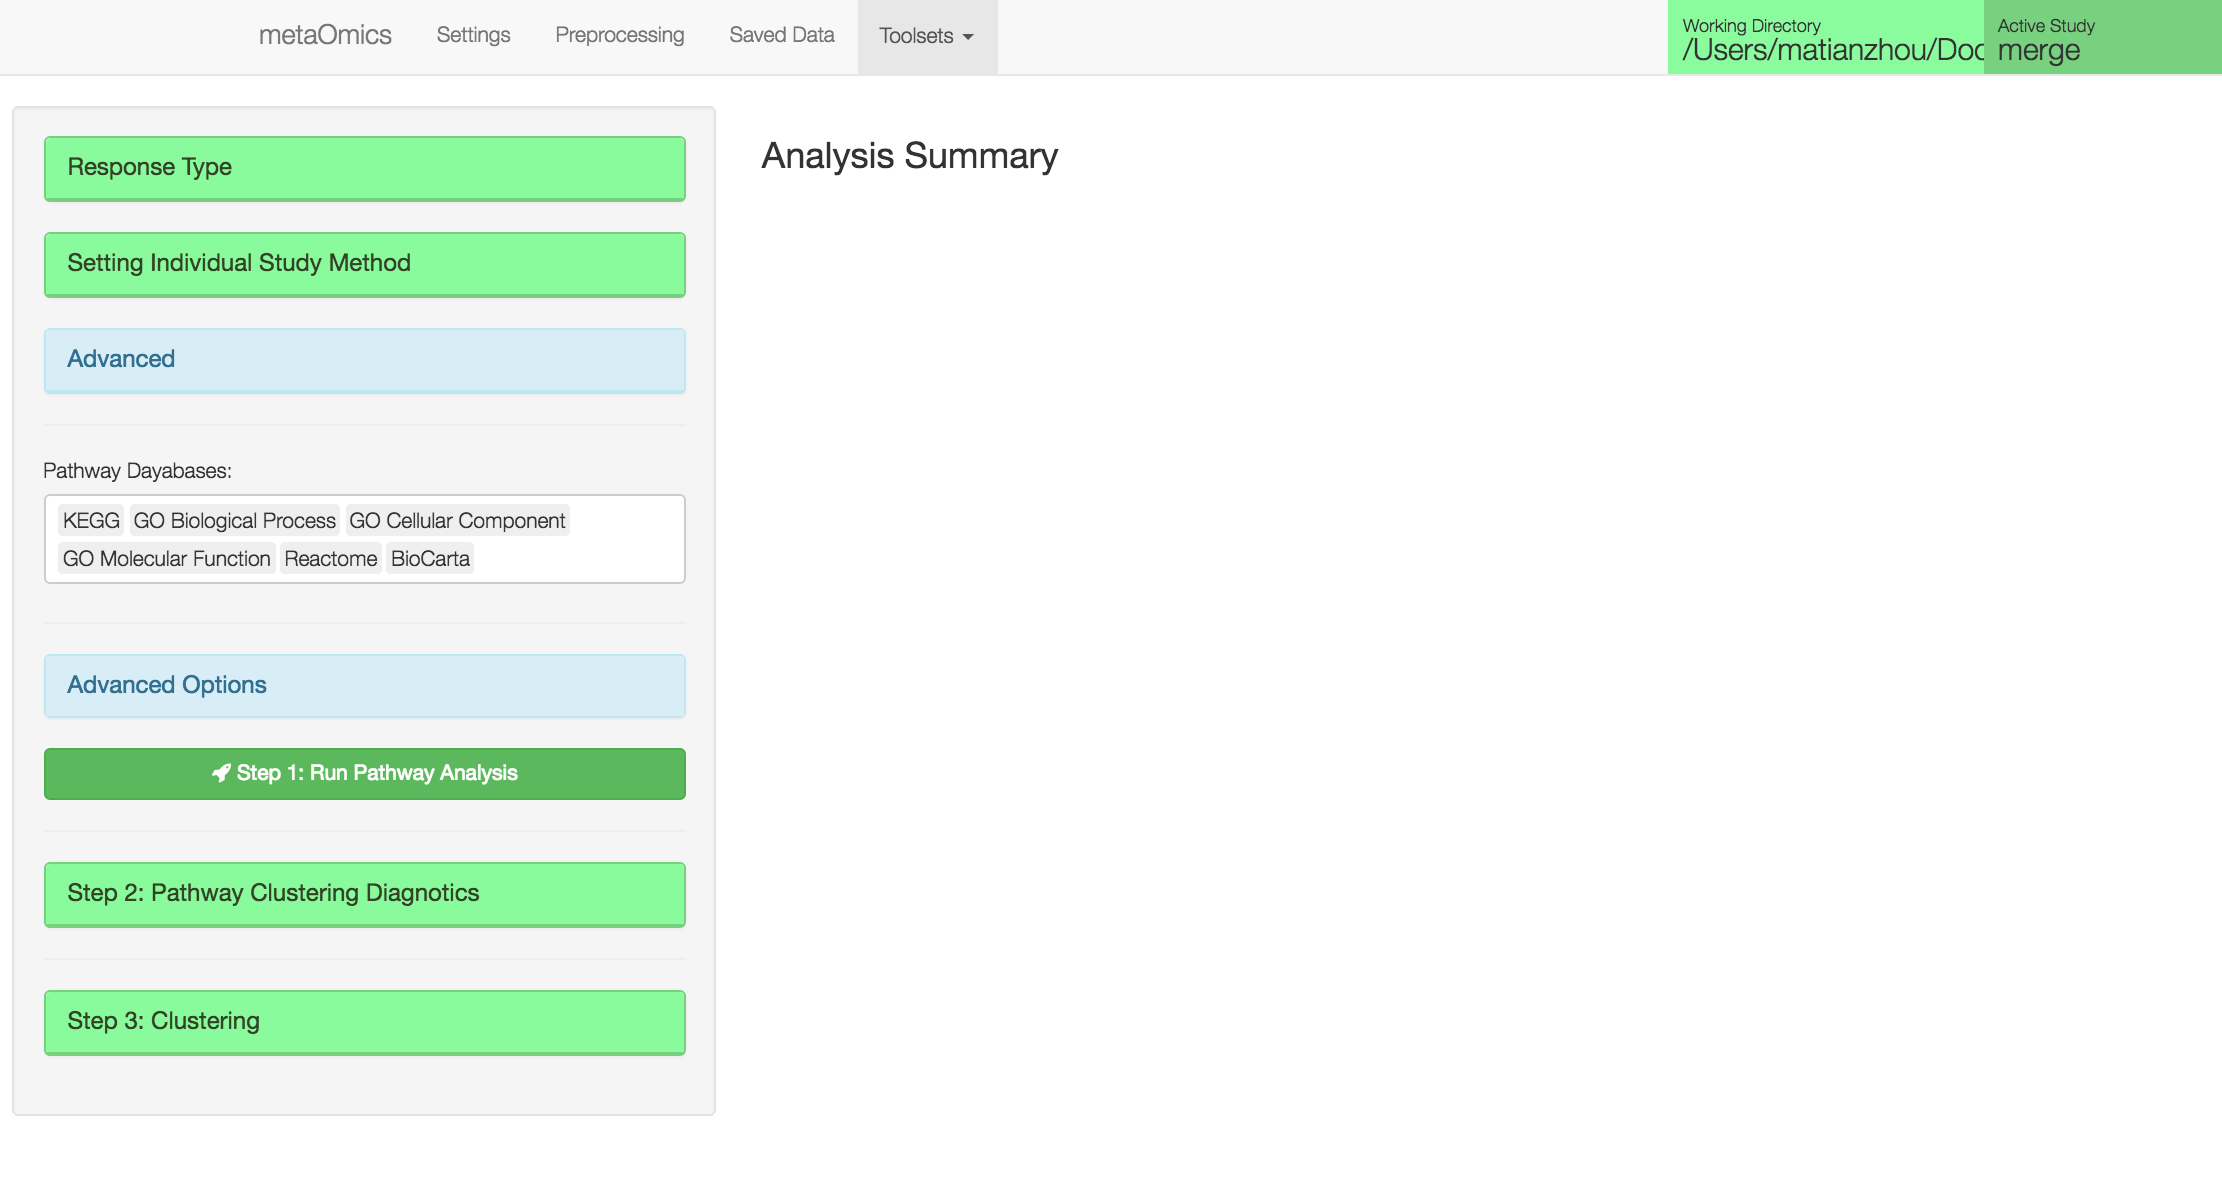
\includegraphics[scale=0.35]{./figure/metaPath/MetaPathmainpage}
\caption{Homepage of MetaPath}
\label{fig:MetaPathmainpage}
\end{center}
\end{figure}

To start, we need to perform DE (association) analysis in each individual study before performing pathway analysis for functional annotation. We click on ``Response Type", for two-class DE analysis, choose ``Two Class Comparison", choose the group label name for the Label Attribute (from the column names of your clinical data). Then for the group label (a factor of at least two levels), choose a name for the ``Control Label" and ``Experimental Label", respectively (Figure \ref{fig:ResponseType}).

\begin{figure}[H]
\begin{center}
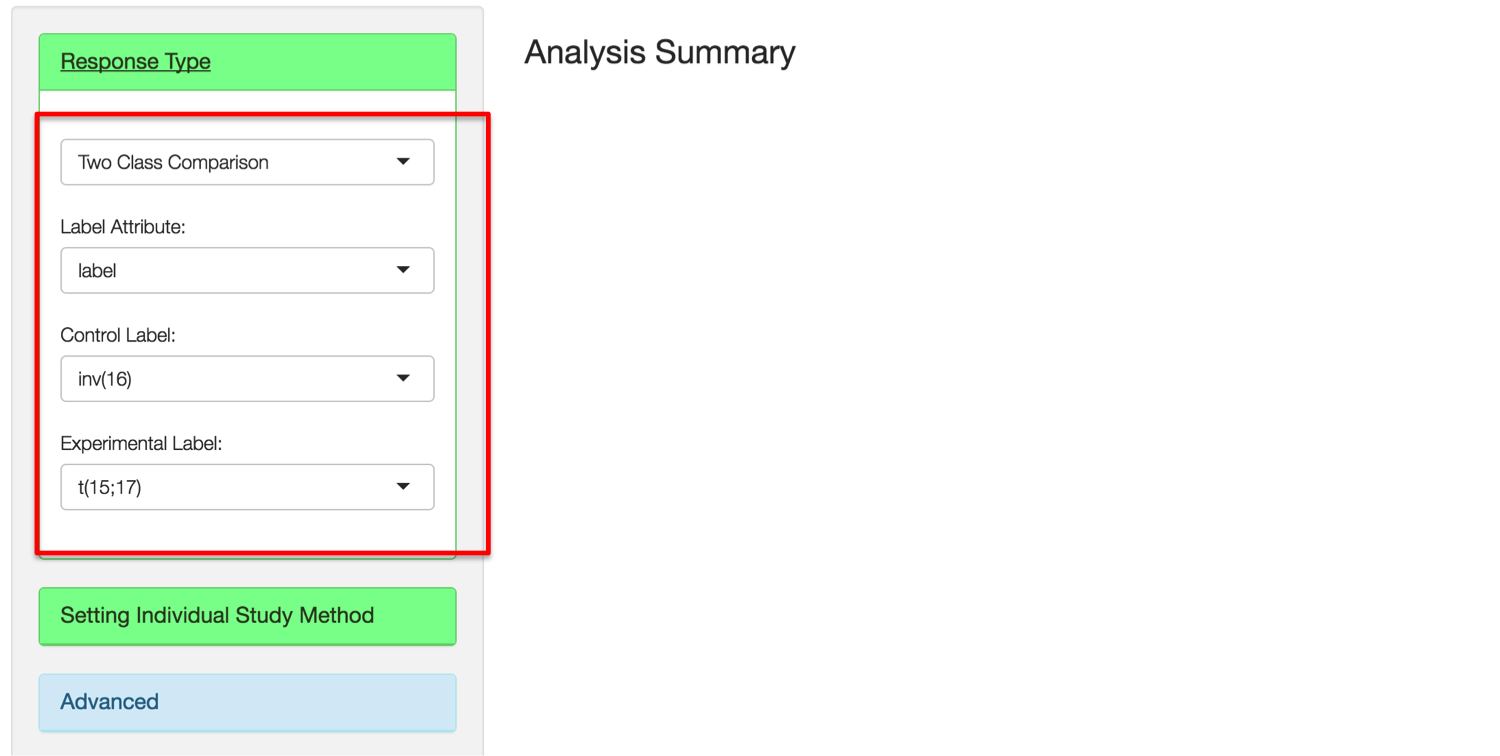
\includegraphics[scale=0.4]{./figure/metaPath/ResponseType}
\caption{Response type setting}
\label{fig:ResponseType}
\end{center}
\end{figure}

Then we click on ``Setting Individual Study Method" and choose ``LIMMA" to perform DE analysis in each individual study (Figure \ref{fig:IndDE}). Available options include ``LIMMA" and ``SAM" for continuous data (e.g. microarray), ``edgeR", ``DESeq2" and ``limmaVoom" for discrete data (e.g. RNA-seq count). Details of the above mentioned DE methods can be found in XXX (reference).

\begin{figure}[H]
\begin{center}

\includegraphics[scale=0.4]{./figure/metaPath/IndDE}
\caption{Individual study DE analysis method}
\label{fig:IndDE}
\end{center}
\end{figure}

Optionally, we can click on ``Advanced" and choose whether to adjust for any important ``Covariates" (e.g. potential confounders) and we set the alternative hypothesis to be ``abs", i.e. two-sided test (Figure \ref{fig:Adv}). 

\begin{figure}[H]
\begin{center}
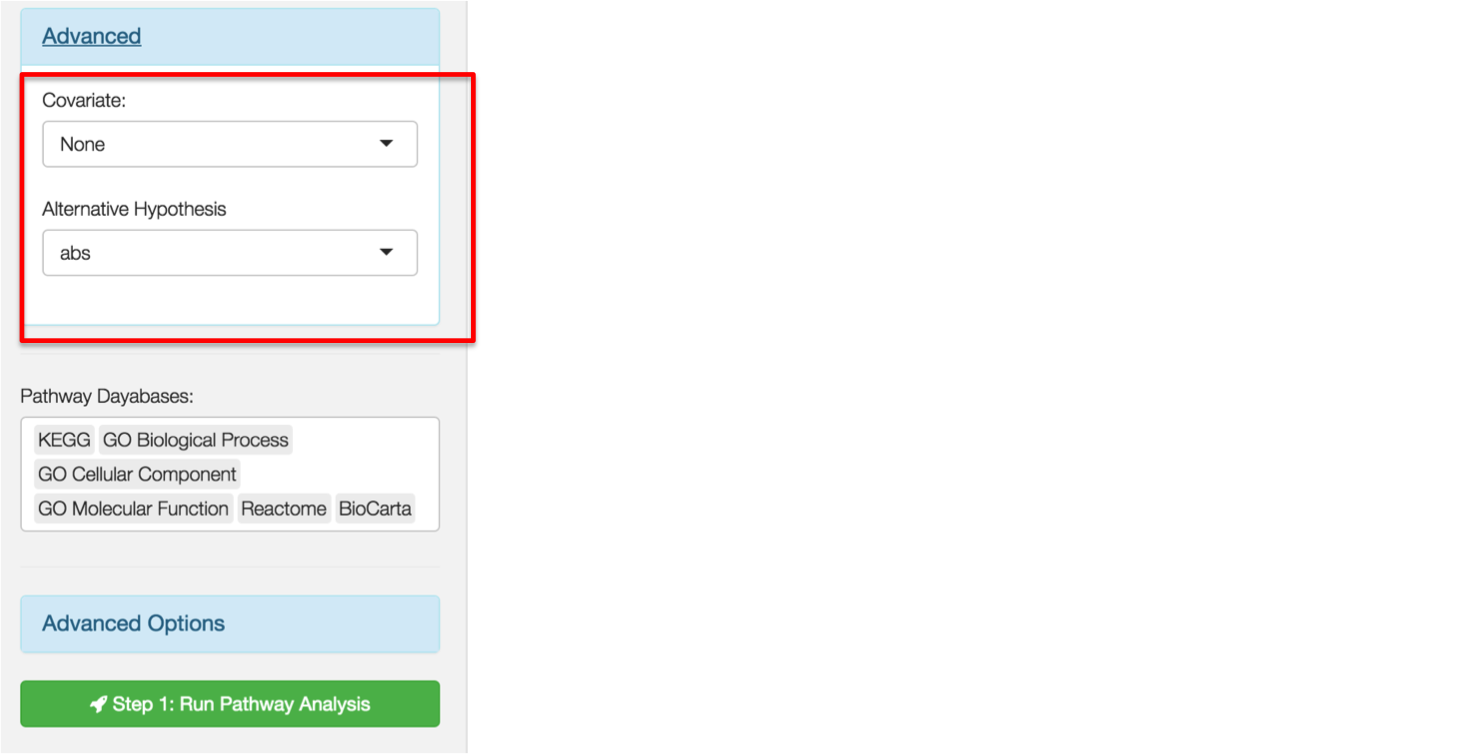
\includegraphics[scale=0.4]{./figure/metaPath/Adv}
\caption{Advanced Options for single study association analysis}
\label{fig:Adv}
\end{center}
\end{figure}

Next, we need to specify the parameters for pathway analysis. As shown in Figure \ref{fig:PathwayDB}, we first need to choose the Pathway databases to be used as shown in the highlighted box. Then optionally, we can click on the ``Advanced Options" tab and choose the software to be used: CPI or MAPE. For CPI, we can use the Kolmogorov-Smirnov test (Figure \ref{fig:CPI}).CPI implements AW Fisher's method for meta p-value method in order to see both consensus and differential enrichment patterns. Alternatively, one can choose to use Fisher's exact test, once this method is selected, we need to pick the number of top ranked genes as the DE gene set for pathway analysis (Figure \ref{fig:FisherExact}). For MAPE, the two tests are also available. There is one additional option of meta p-value method, available options include Fisher's method, maxP, minP, rOP and AW Fisher' method (Figure \ref{fig:MAPE}). When rOP is selected, additional option for order statistic of p-value (rth ordered p-value) will be available. Instead of closed-form distributions, users can use permutation of gene labels to get pathway p-value forthe Kolmogorov-Smirnov test (Figure \ref{fig:MAPE}). When ``Permutation to get p-value" is choosen to be ``YES", additional option for number of permutations will be available. However, we generally suggest users not to run permutation because it may take up to hours to compute. Lastly, we will specify the minimum/maximum pathway size of pathways we wish to include for functional analysis, then click ``Step 1: Run Pathway Analysis".     

\begin{figure}[H]
\begin{center}
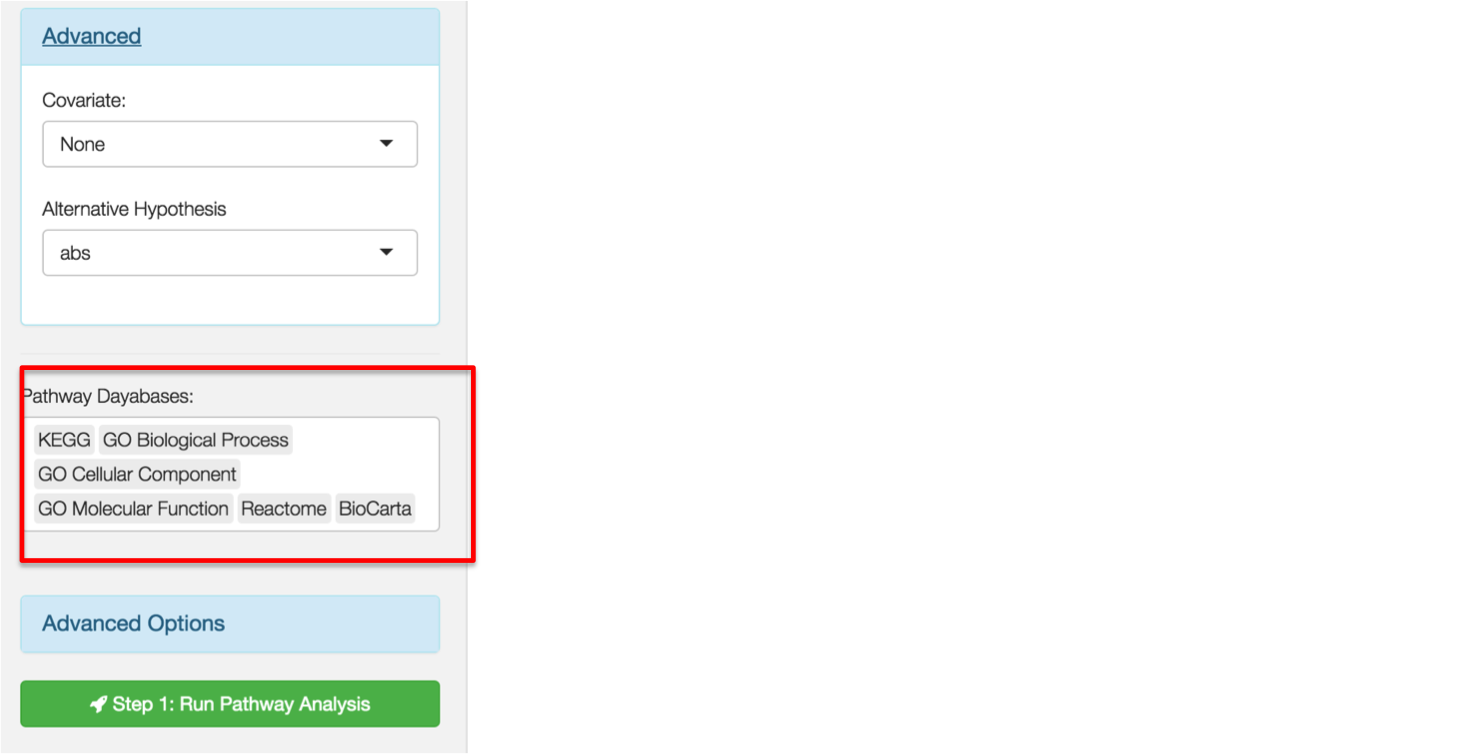
\includegraphics[scale=0.45]{./figure/metaPath/PathwayDB}
\caption{Selection of pathway database}
\label{fig:PathwayDB}
\end{center}
\end{figure}

\begin{figure}[H]
\begin{center}
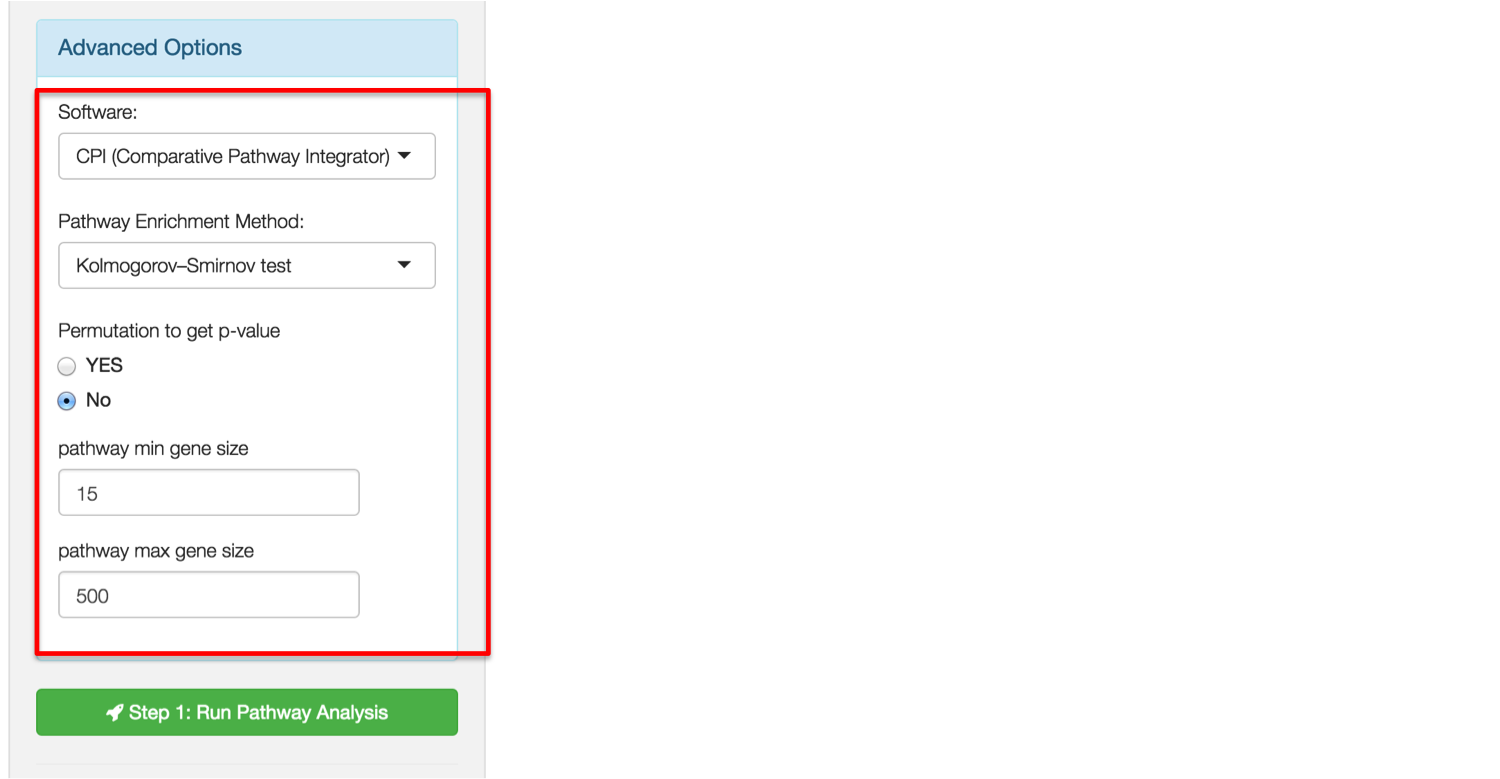
\includegraphics[scale=0.45]{./figure/metaPath/CPI}
\caption{CPI setting}
\label{fig:CPI}
\end{center}
\end{figure}

\begin{figure}[H]
\begin{center}
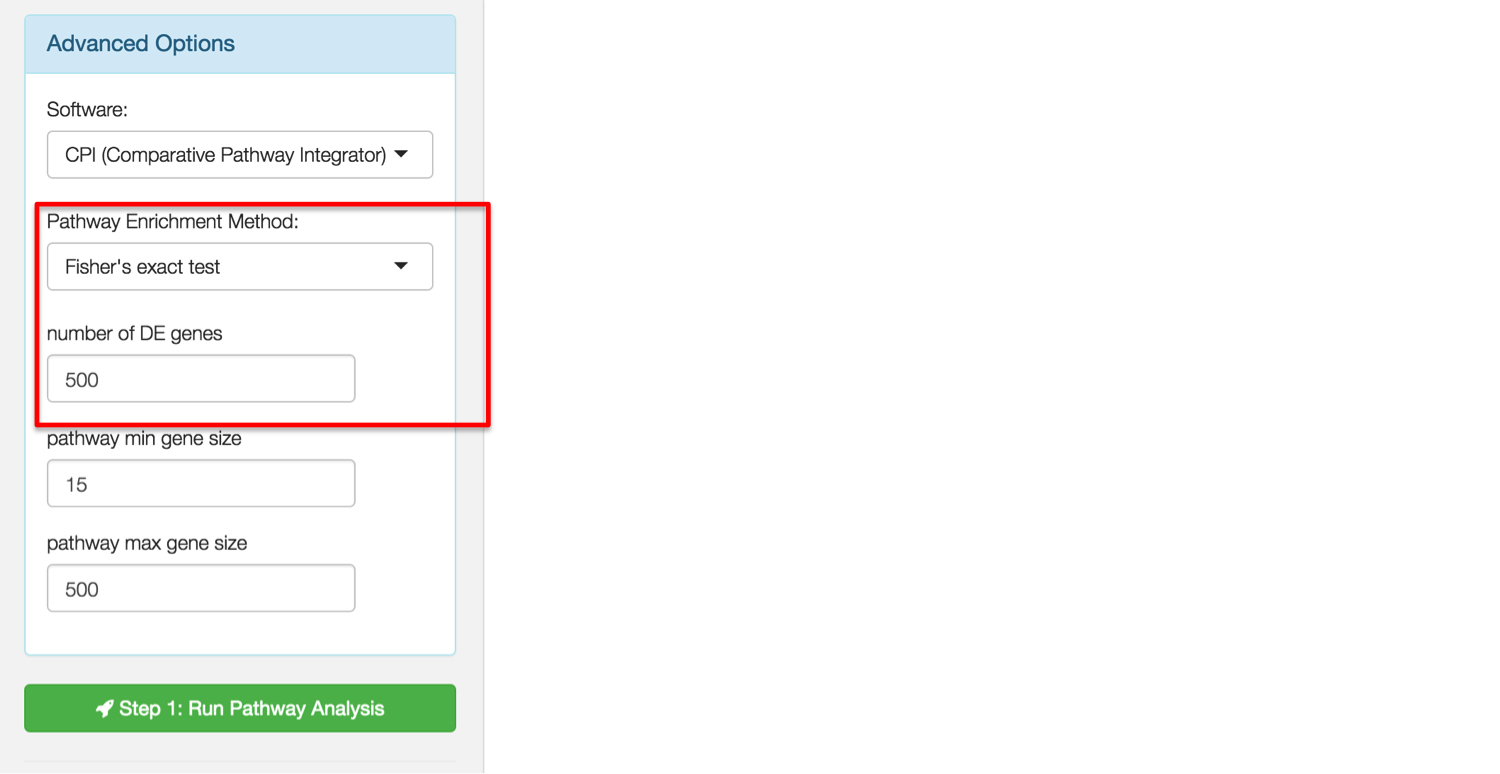
\includegraphics[scale=0.45]{./figure/metaPath/FisherExact}
\caption{Fisher's Exact Test}
\label{fig:FisherExact}
\end{center}
\end{figure}

\begin{figure}[H]
\begin{center}
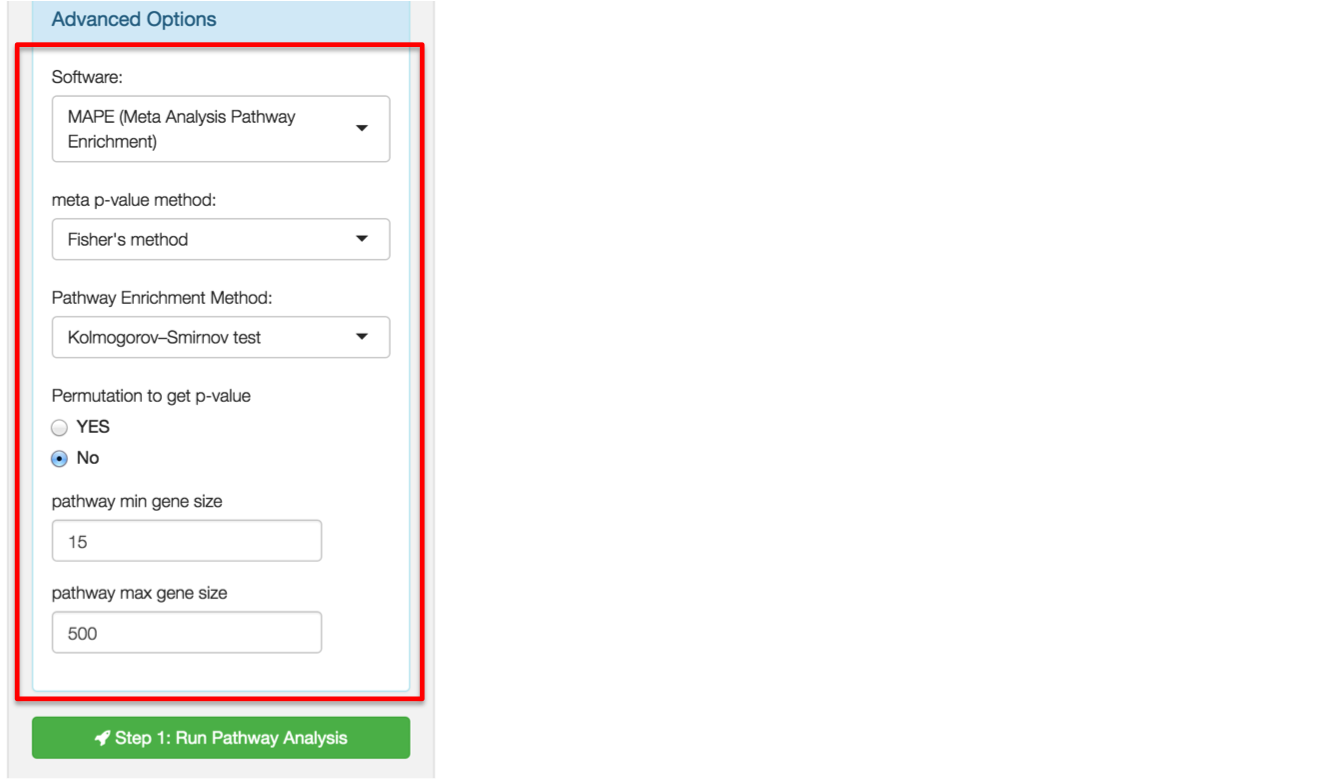
\includegraphics[scale=0.45]{./figure/metaPath/MAPE}
\caption{MAPE setting}
\label{fig:MAPE}
\end{center}
\end{figure}

We will see a summary table generated on the right of the page as shown in Figure \ref{fig:CPISummary} (based on the default CPI method). The ``Analysis Summary" includes the analysis results of all pathways, including individual study association analysis p-value, meta pathway analysis p-value/FDR, etc. Users can search the gene name in the ``Search" bar, and the full table is automatically saved in the working directory specified before.  

\begin{figure}[H]
\begin{center}
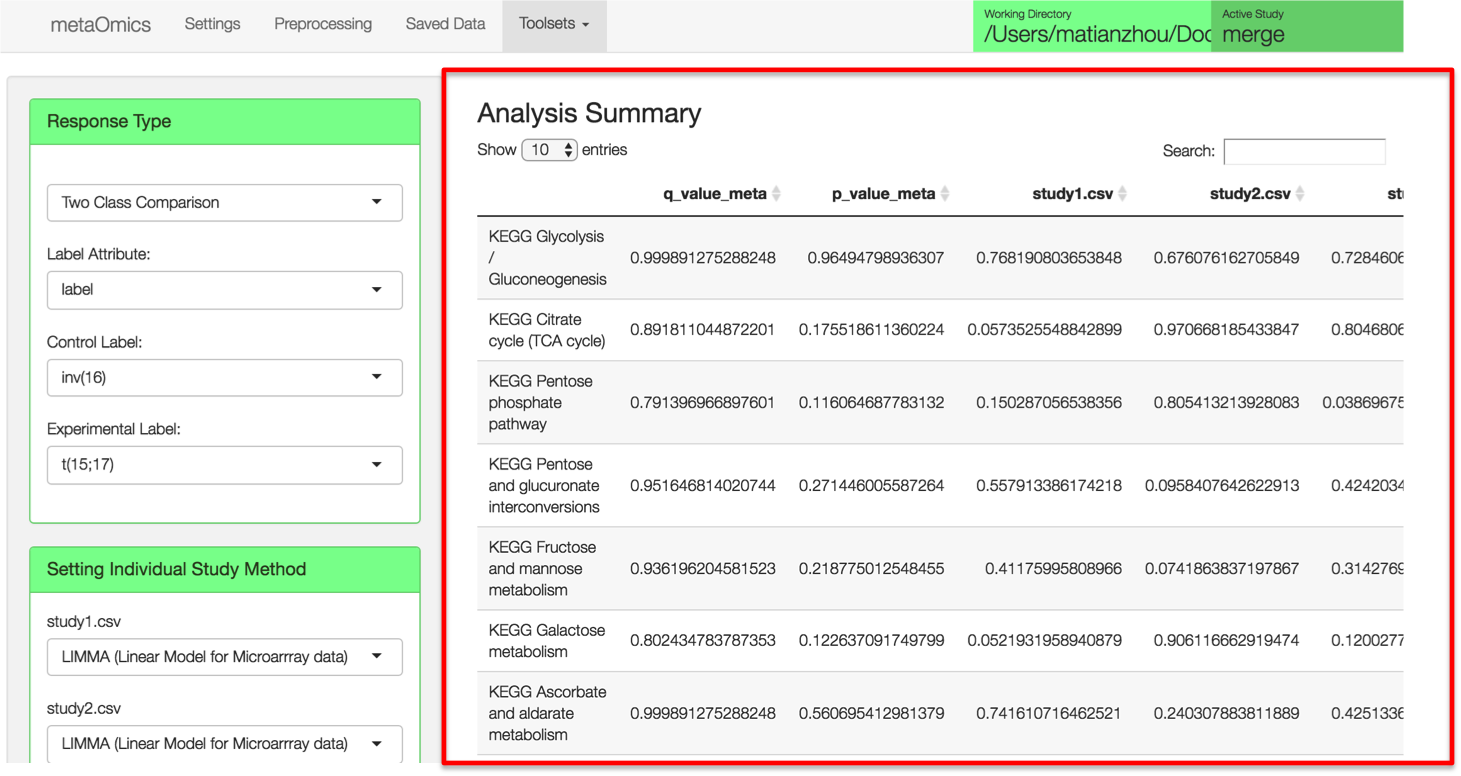
\includegraphics[scale=0.45]{./figure/metaPath/CPISummary}
\caption{Summary table of CPI analysis results}
\label{fig:CPISummary}
\end{center}
\end{figure}

\subsubsection{Pathway clustering}

In the next step, we performed clustering diagnostics of pathways at specified FDR cutoff (Figure \ref{fig:ClustDiag}). After clicking on ``Pathway Cluster Diagnostics", we will see two plots generated on the right panel: consensus CDF and Delta area plots (Figure \ref{fig:DiagPlots}), we can use these two plots to determine the optimal number of clusters, to be used in the third clustering step.  

\begin{figure}[H]
\begin{center}
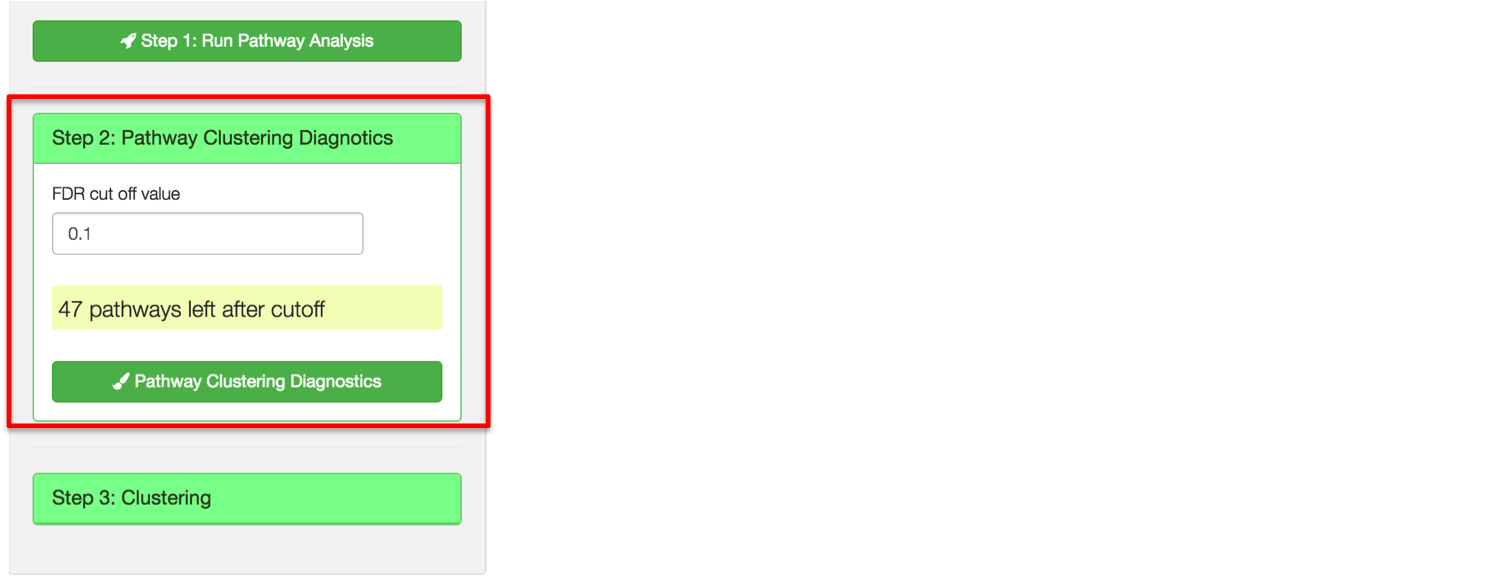
\includegraphics[scale=0.45]{./figure/metaPath/ClustDiag}
\caption{Pathway clustering diagnostics}
\label{fig:ClustDiag}
\end{center}
\end{figure}

\begin{figure}[H]
\begin{center}
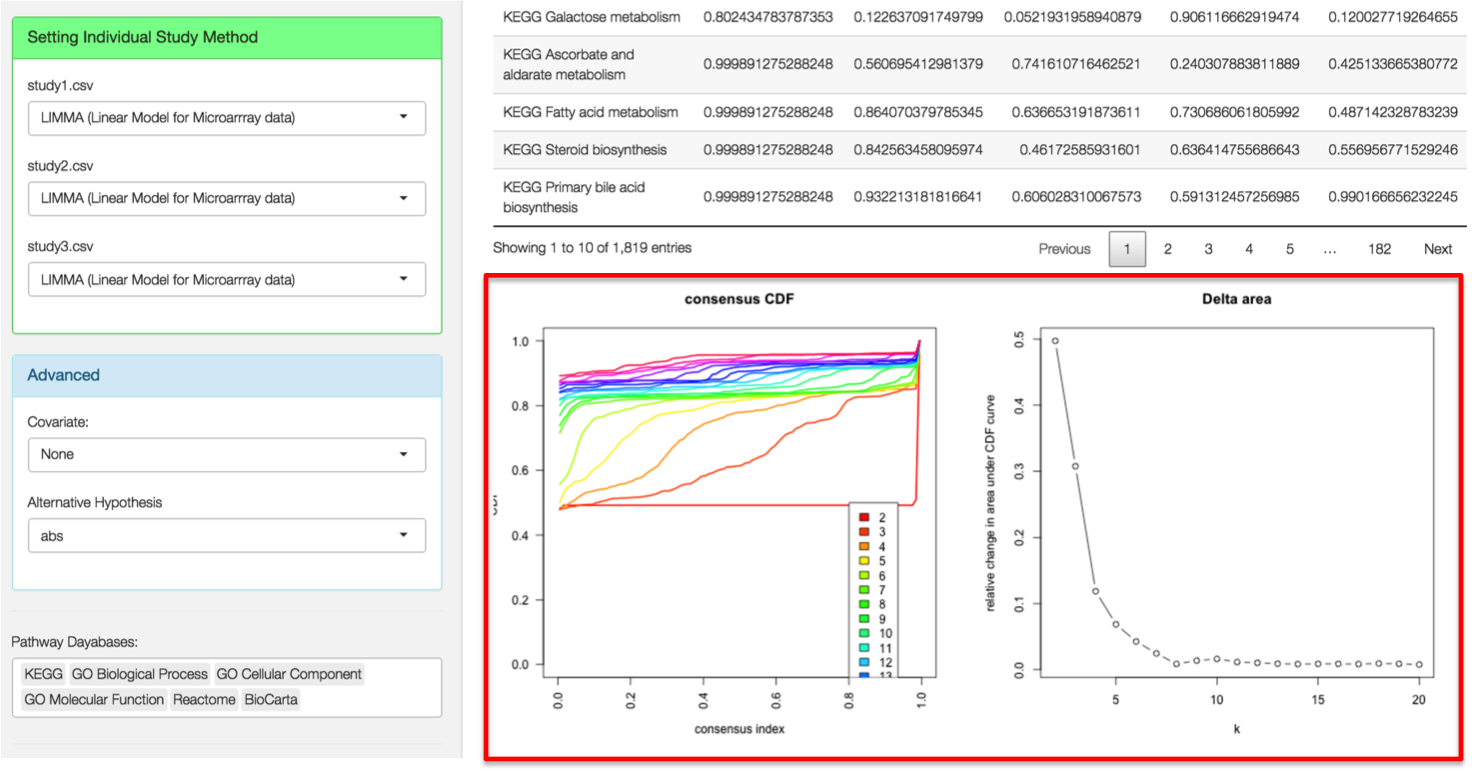
\includegraphics[scale=0.45]{./figure/metaPath/DiagPlots}
\caption{Diagnostic plots}
\label{fig:DiagPlots}
\end{center}
\end{figure}
